\section{The OrbitDB Field Manual}\label{the-orbitdb-field-manual}

Readme TBD \emph{Note:} Please see the \href{./README.md}{README} before
beginning this chapter.

\section{Tutorial Chapter 1 - Laying the
Foundation}\label{tutorial-chapter-1---laying-the-foundation}

\begin{quote}
The basics of OrbitDB include undertanding how to \emph{install OrbitDB
(and IPFS)}, \emph{create a new databases}, and how \emph{addressing}
works.
\end{quote}

\subsection{Instantiating OrbitDB}\label{instantiating-orbitdb}

Start by installing OrbitDB and its dependency, IPFS. The process is
different between the browser and node.js, so we cover both here.

\subsubsection{Installation in Node.js}\label{installation-in-node.js}

Choose a project directory and \texttt{cd} to there from your command
line:

From the command line:

\begin{Shaded}
\begin{Highlighting}[]
\NormalTok{$ }\ExtensionTok{npm}\NormalTok{ install orbitdb ipfs}
\end{Highlighting}
\end{Shaded}

Then, in your script, require the modules:

\begin{Shaded}
\begin{Highlighting}[]
\KeywordTok{const}\NormalTok{ Ipfs }\OperatorTok{=} \AttributeTok{require}\NormalTok{(}\StringTok{'ipfs'}\NormalTok{)}
\KeywordTok{const}\NormalTok{ OrbitDB }\OperatorTok{=} \AttributeTok{require}\NormalTok{(}\StringTok{'orbit-db'}\NormalTok{)}
\end{Highlighting}
\end{Shaded}

\subsubsection{Installation in the
Browser}\label{installation-in-the-browser}

For the purposes of this tutorial, we recommend using unpkg for
obtaining pre-built, minified versions of both IPFS and OrbitDB. Simply
include these at the top of your \texttt{index.html} file:

\begin{Shaded}
\begin{Highlighting}[]
\KeywordTok{<script}\OtherTok{ src=}\StringTok{"https://unpkg.com/ipfs/dist/index.min.js"}\KeywordTok{></script>}
\KeywordTok{<script}\OtherTok{ src=}\StringTok{"https://www.unpkg.com/orbit-db/src/OrbitDB.js"}\KeywordTok{></script>}
\end{Highlighting}
\end{Shaded}

There are other ways to get this code, including building it yourself.
We detail these in Part 3.

\subsection{Standing up IPFS and
OrbitDB}\label{standing-up-ipfs-and-orbitdb}

We have designed Chapters 1 and 2 of the tutorial to work work offline,
not requiring any internet connectivity or connections to peers.

OrbitDB requires a running IPFS node to operate, so you will create one
here and notify OrbitDB about it. by running the following code.

\begin{Shaded}
\begin{Highlighting}[]
\KeywordTok{let}\NormalTok{ orbitdb}

\KeywordTok{let}\NormalTok{ node }\OperatorTok{=} \KeywordTok{new} \AttributeTok{Ipfs}\NormalTok{(}\OperatorTok{\{}
  \DataTypeTok{preload}\OperatorTok{:} \OperatorTok{\{} \DataTypeTok{enabled}\OperatorTok{:} \KeywordTok{false} \OperatorTok{\},}
  \DataTypeTok{repo}\OperatorTok{:} \StringTok{"./ipfs"}\OperatorTok{,}
  \DataTypeTok{EXPERIMENTAL}\OperatorTok{:} \OperatorTok{\{} \DataTypeTok{pubsub}\OperatorTok{:} \KeywordTok{true} \OperatorTok{\},}
  \DataTypeTok{config}\OperatorTok{:} \OperatorTok{\{}
    \DataTypeTok{Bootstrap}\OperatorTok{:}\NormalTok{ []}\OperatorTok{,}
    \DataTypeTok{Addresses}\OperatorTok{:} \OperatorTok{\{} \DataTypeTok{Swarm}\OperatorTok{:}\NormalTok{ [] }\OperatorTok{\}}
  \OperatorTok{\}}
\OperatorTok{\}}\NormalTok{)}\OperatorTok{;}

\VariableTok{node}\NormalTok{.}\AttributeTok{on}\NormalTok{(}\StringTok{"error"}\OperatorTok{,}\NormalTok{ (e) }\OperatorTok{=>} \OperatorTok{\{} \ControlFlowTok{throw} \KeywordTok{new} \AttributeTok{Error}\NormalTok{(e) }\OperatorTok{\}}\NormalTok{)}
\VariableTok{node}\NormalTok{.}\AttributeTok{on}\NormalTok{(}\StringTok{"ready"}\OperatorTok{,} \AttributeTok{async}\NormalTok{ () }\OperatorTok{=>} \OperatorTok{\{}
\NormalTok{  orbitdb }\OperatorTok{=}\NormalTok{ await }\VariableTok{OrbitDB}\NormalTok{.}\AttributeTok{createInstance}\NormalTok{(node)}
  \VariableTok{console}\NormalTok{.}\AttributeTok{log}\NormalTok{(}\VariableTok{orbitdb}\NormalTok{.}\AttributeTok{id}\NormalTok{)}
\OperatorTok{\}}\NormalTok{)}
\end{Highlighting}
\end{Shaded}

In the output you will see something called a ``multihash'', like
\texttt{QmPSicLtjhsVifwJftnxncFs4EwYTBEjKUzWweh1nAA87B}. For now, just
know that this is the identifier of your IPFS node. We explain
multihashes in more detail in \textbf{Part 2: Peer-to-Peer}

\subsubsection{What just happened?}\label{what-just-happened}

Starting with the \texttt{new\ Ipfs} line, your code creates a new IPFS
node. Note the default settings:

\begin{itemize}
\tightlist
\item
  \texttt{preload:\ \{\ enabled:\ false\ \}} disables the use of
  so-called ``pre-load'' IPFS nodes. These nodes exist to help load
  balance the global network and prevent DDoS. However, these nodes can
  go down and cause errors. Since we are only working offline for now,
  we include this line to disable them.
\item
  \texttt{repo:\ \textquotesingle{}./ipfs\textquotesingle{}} designates
  the path of the repo in node.js only. In the browser, you can actually
  remove this line. The default setting is a folder called
  \texttt{.jsipfs} in your home directory. You will see why we choose
  this acute location for the folder later.
\item
  \texttt{XPERIMENTAL:\ \{\ pubsub:\ true\ \}} enables IPFS pubsub,
  which is a method of communicating between nodes and is required for
  OrbitDB usage, despite whether or not we are connected to other peers.
\item
  \texttt{config:\ \{\ Bootstrap:\ {[}{]},\ Addresses:\ \{\ Swarm:\ {[}{]}\ \}\}}
  sets both our bootstrap peers list (peers that are loaded on
  instantiation) and swarm peers list (peers that can connect and
  disconnect at any time to empty. We will populate these later.
\item
  \texttt{node.on("error",\ (e)\ =\textgreater{}\ \{\ throw\ new\ Error(e)\ \})}
  implements extremely basic error handling for if something happens
  during node creation
\item
  \texttt{node.on("ready",\ (e)\ =\textgreater{}\ \{\ orbitdb\ =\ new\ OrbitDB(node)\ \})}
  instantiates OrbitDB on top of the IPFS node, when it is ready.
\end{itemize}

By running the code above, you have created a new IPFS node that works
locally and is not connected to any peers. You have also loaded a new
\texttt{orbitdb} object into memory, ready to create databases and
manage data.

\emph{You are now ready to use OrbitDB!}

\begin{itemize}
\tightlist
\item
  Resolves \#\href{https://github.com/orbitdb/orbit-db/issues/367}{367}
\end{itemize}

\paragraph{What else happened in
node.js?}\label{what-else-happened-in-node.js}

When you ran the code in node.js, you created two folders in your
project structure: \texttt{\textquotesingle{}orbitdb/} and
\texttt{ipfs/}.

\begin{Shaded}
\begin{Highlighting}[]
\NormalTok{$ }\CommentTok{# slashes added to ls output for effect}
\NormalTok{$ }\FunctionTok{ls}\NormalTok{ orbitdb/}
\ExtensionTok{QmNrPunxswb2Chmv295GeCvK9FDusWaTr1ZrYhvWV9AtGM/}

\NormalTok{$ }\FunctionTok{ls}\NormalTok{ ipfs/}
\ExtensionTok{blocks/}\NormalTok{  config  datastore/  datastore_spec  keys/  version}
\end{Highlighting}
\end{Shaded}

Focusing your attention on the IPFS folder, you will see that the
subfolder has the same ID as orbitdb. This is purposeful, as this
initial folder contains metadata that OrbitDB will need to operate. For
now let's not go into detail

The \texttt{ipfs/} folder contains all of your IPFS data. Explaining
this in depth is outside of the scope of this tutorial, and the curious
can find out more \protect\hyperlink{}{here}.

\paragraph{What else happened in the
browser?}\label{what-else-happened-in-the-browser}

In the browser IPFS content is handled inside of IndexedDB, a persistent
storage mechanism for browsers

\hypertarget{}{
\begin{figure}
\centering
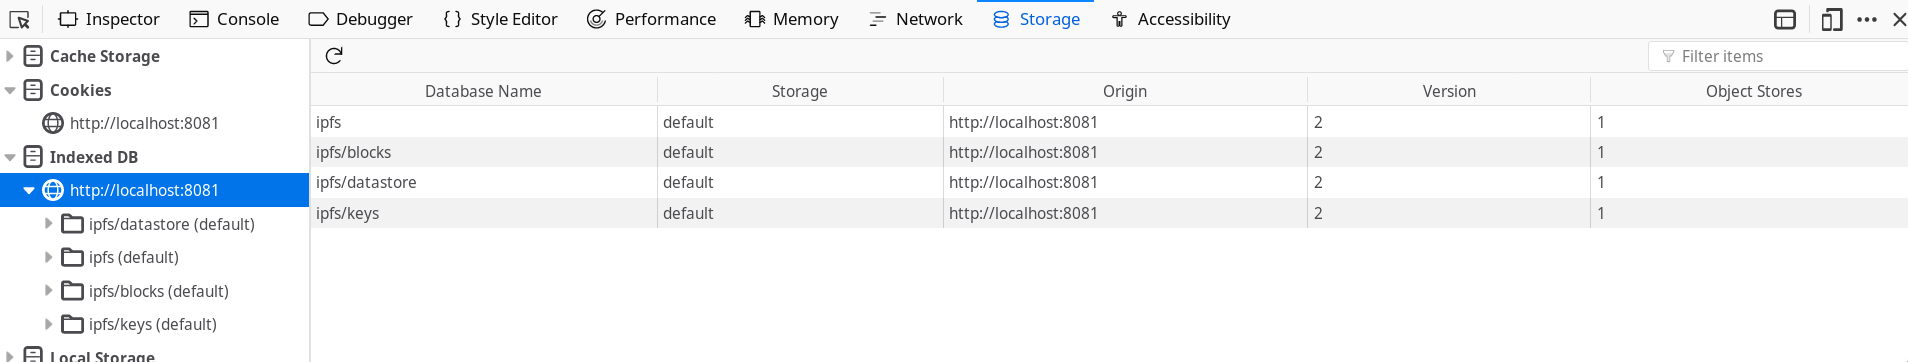
\includegraphics{../images/ipfs_browser.png}
\caption{alt browser whatever}
\end{figure}
}

Note since you have not explicitly defined a database in the broser, no
IndexedDB databases have been created for OrbitDB yet.

\textbf{Caution!} iOS and Android have been known to purge IndexedDB if
storage space needs to be created inside of your phone. We recommend
creating robust backup mechanisms at the application layer.

\hypertarget{creating-a-database}{\subsection{Creating a
Database}\label{creating-a-database}}

Now you will create a local database that *only you8 can read.

Remember the code snippet from above, starting and ending with:

\begin{Shaded}
\begin{Highlighting}[]
\KeywordTok{let}\NormalTok{ orbitdb}

\CommentTok{/* ... */}

\VariableTok{node}\NormalTok{.}\AttributeTok{on}\NormalTok{(}\StringTok{"ready"}\OperatorTok{,} \AttributeTok{async}\NormalTok{ () }\OperatorTok{=>} \OperatorTok{\{}
\NormalTok{  orbitdb }\OperatorTok{=} \KeywordTok{new} \VariableTok{OrbitDB}\NormalTok{.}\AttributeTok{createInstance}\NormalTok{(node)}
  \VariableTok{console}\NormalTok{.}\AttributeTok{log}\NormalTok{(}\VariableTok{orbitdb}\NormalTok{.}\AttributeTok{id}\NormalTok{)}
\OperatorTok{\}}\NormalTok{)}
\end{Highlighting}
\end{Shaded}

Expand that to the following, and then run the code:

\begin{Shaded}
\begin{Highlighting}[]
\KeywordTok{let}\NormalTok{ orbitdb}\OperatorTok{,}\NormalTok{ pieces}

\CommentTok{/* ... */}

\VariableTok{node}\NormalTok{.}\AttributeTok{on}\NormalTok{(}\StringTok{"ready"}\OperatorTok{,} \AttributeTok{async}\NormalTok{ () }\OperatorTok{=>} \OperatorTok{\{}
\NormalTok{  orbitdb }\OperatorTok{=}\NormalTok{ await }\VariableTok{OrbitDB}\NormalTok{.}\AttributeTok{createInstance}\NormalTok{(node)}

  \KeywordTok{const}\NormalTok{ options }\OperatorTok{=} \OperatorTok{\{}
    \DataTypeTok{accessController}\OperatorTok{:} \OperatorTok{\{} \DataTypeTok{write}\OperatorTok{:}\NormalTok{ [}\VariableTok{orbitdb}\NormalTok{.}\VariableTok{identity}\NormalTok{.}\AttributeTok{publicKey}\NormalTok{] }\OperatorTok{\}}
    \DataTypeTok{indexBy}\OperatorTok{:} \StringTok{"hash"}
  \OperatorTok{\}}
  
\NormalTok{  pieces }\OperatorTok{=}\NormalTok{ await }\VariableTok{orbitdb}\NormalTok{.}\AttributeTok{docstore}\NormalTok{(}\StringTok{'pieces'}\OperatorTok{,}\NormalTok{ options)}
\NormalTok{  await }\VariableTok{pieces}\NormalTok{.}\AttributeTok{load}\NormalTok{()}
  
\NormalTok{  pieces }\OperatorTok{=} \VariableTok{piecesDb}\NormalTok{.}\AttributeTok{get}\NormalTok{(}\StringTok{'all'}\NormalTok{)}
  \VariableTok{console}\NormalTok{.}\AttributeTok{log}\NormalTok{(}\VariableTok{pieces}\NormalTok{.}\AttributeTok{address}\NormalTok{)}
\OperatorTok{\}}\NormalTok{)}
\end{Highlighting}
\end{Shaded}

You will see the output of a simple empty array, \texttt{{[}{]}}. We
understand this may not be immediately impressive, but a lot of
important things quietly happened.

\subsubsection{What just happened?}\label{what-just-happened-1}

Your code created a new database, of type ``docstore'', writable only by
you.

\begin{itemize}
\tightlist
\item
  The \texttt{options} defines the paramaters for the database we are
  about to create.
\item
  \texttt{accessController:\ \{\ write:\ {[}orbitdb.identity.publicKey{]}\ \}}
  defines the ACL, or ``Access Control List''. In this instance we are
  restricting \texttt{write} access to ONLY orbitdb instances identified
  by our particular \texttt{publicKey}
\item
  \texttt{indexBy:\ "hash"} is a docstore-specific option, which
  specifies which field to index our database by
\item
  \texttt{pieces\ =\ await\ orbitdb.docstore(\textquotesingle{}pieces\textquotesingle{},\ options)}
  is the magic line that creates the database. Once this line is
  completed, the database is open and can be acted upon.
\end{itemize}

\textbf{Caution!} A note about identity: Your public key is not your
identity. We repeat, \emph{your public key is not your identity}.
Though, it is often used as such for convenience's sake, and the lack of
better alternatives. So, in the early parts of this tutorial we say
``writable only to you'' when we really mean ``writable only by an
OrbitDB instance on top of an IPFS node that has the correct id, which
we are assuming is controlled by you.''

See for more info:
https://github.com/orbitdb/orbit-db/blob/525978e0a916a8b027e9ea73d8736acb2f0bc6b4/src/OrbitDB.js\#L106

\begin{itemize}
\tightlist
\item
  Resolves \#\href{https://github.com/orbitdb/orbit-db/issues/366}{366}
\item
  Resolves \#\href{https://github.com/orbitdb/orbit-db/issues/502}{502}
\end{itemize}

\paragraph{What else happened in
node.js?}\label{what-else-happened-in-node.js-1}

\paragraph{What else happened in the
browser?}\label{what-else-happened-in-the-browser-1}

\subsection{Addressing}\label{addressing}

This section isn't necessarily a hands-on part of the tutorial, but it's
incredibly important

\subsection{Reading and Writing Data}\label{reading-and-writing-data}

\begin{quote}
Potentially split out to chapter 2?
\end{quote}

\begin{itemize}
\tightlist
\item
  Resolves \#\href{https://github.com/orbitdb/orbit-db/issues/365}{365}
\item
  Resolves \#\href{https://github.com/orbitdb/orbit-db/issues/438}{438}
\item
  Resolves \#\href{https://github.com/orbitdb/orbit-db/issues/381}{381}
\item
  Resolves \#\href{https://github.com/orbitdb/orbit-db/issues/242}{242}
\item
  Resolves \#\href{https://github.com/orbitdb/orbit-db/issues/430}{430}
  \#\# Chapter 2: Peer-to-Peer
\end{itemize}

\subsubsection{Replication Overview}\label{replication-overview}

\begin{itemize}
\tightlist
\item
  Resolves \#\href{https://github.com/orbitdb/orbit-db/issues/463}{463}
\item
  Resolves \#\href{https://github.com/orbitdb/orbit-db/issues/468}{468}
\item
  Resolves \#\href{https://github.com/orbitdb/orbit-db/issues/471}{471}
\item
  Resolves \#\href{https://github.com/orbitdb/orbit-db/issues/498}{498}
\item
  Resolves \#\href{https://github.com/orbitdb/orbit-db/issues/519}{519}
\item
  Resolves \#\href{https://github.com/orbitdb/orbit-db/issues/296}{296}
\item
  Resolves \#\href{https://github.com/orbitdb/orbit-db/issues/264}{264}
\item
  Resolves \#\href{https://github.com/orbitdb/orbit-db/issues/460}{460}
\item
  Resolves \#\href{https://github.com/orbitdb/orbit-db/issues/484}{484}
\item
  Resolves \#\href{https://github.com/orbitdb/orbit-db/issues/474}{474}
\item
  Resolves \#\href{https://github.com/orbitdb/orbit-db/issues/505}{505}
\end{itemize}

\subsubsection{Replicating in the
Browser}\label{replicating-in-the-browser}

\subsubsection{Replicating in Node.js}\label{replicating-in-node.js}

\subsubsection{Replication between Browser and
Node.js}\label{replication-between-browser-and-node.js}

\begin{itemize}
\tightlist
\item
  Resolves \#\href{https://github.com/orbitdb/orbit-db/issues/496}{496}
  \# The OrbitDB Tutorial
\end{itemize}

\begin{quote}
An interactive, imperative adventure of peer-to-peer, decentralized, and
distributed proportions
\end{quote}

\subsection{Requirements}\label{requirements}

\begin{itemize}
\tightlist
\item
  A computer
\item
  A command line (unix/linux based or windows command prompt)
\item
  A modern web browser (Firefox, Chrome, Edge, etc)
\item
  Node.js installed
\end{itemize}

\subsection{What will I build?}\label{what-will-i-build}

You will build an app that provides royalty-free sheet music on-demand
for musicians, based on their instrument.

You will access a global catalog of royalty-free sheet music. Then,
given an instrument name as input (Violin, Saxophone, Marimba) you it
will display piece of sheet music at random. Futhermore, you will give
the users the ability to submit their own music and share it with
connected peers.

You will use OrbitDB as the backbone for this, creating a few databases:
1. The ``global'' starter database of royalty free pieces for all to use
(read only) 2. The user database of pieces they can upload - private

You will write JavaScript and create the backbone of a full application
using OrbitDB in both the browser and on the command line. For the sake
of keeping things focused, we will exclude any HTML or CSS from this
tutorial and focus only on the Javascript code.

\subsubsection{Why a music app?}\label{why-a-music-app}

OrbitDB is already used all over the world, and this tutorial music
reflect that. There are other many topics we could have chosen that
touch the vast majority of humans on earth: finance, politics, climate,
religion. However, those are generally contentious and complicated.

We believe that \textbf{music} is a uniquely universal cultural feature
- something that we more humans than any other topic share, enjoy, or at
least appreciate. Your participation in this tutorial will make it
easier for musicians all over the world to find sheet music to practice
with.

\subsection{Conventions}\label{conventions}

\begin{itemize}
\tightlist
\item
  Read this tutorial in order, the learning builds on itself other over
  time.
\item
  You will switch between writing and reading code, and \emph{What Just
  Happened} sections that explain in depth what happens on a technical
  level when the code is run.
\item
  OrbitDB works in both node.js and in the browser, and this tutorial
  will not focus on one or the other. Stay on your toes.
\item
  This tutorial is not only OS-agnostic and editor-agnostic, it's also
  folder structure agnostic. All of the code examples are designed to
  work if applied in order, regardless of which js file they are in.
  Thus folder and file names for code are avoided.
\item
  \texttt{async} and \texttt{await} are used prominently. Feel free to
  replace those with explicit \texttt{Promise} objects if you're feeling
  daring.
\end{itemize}

Ready? Let's start with \href{./01_Basics.md}{Chapter 1: The Basics}

\section{The OrbitDB Field Manual}\label{the-orbitdb-field-manual-1}

\begin{quote}
Short Description
\end{quote}

\subsection{Table of Contents}\label{table-of-contents}

\begin{itemize}
\tightlist
\item
  Part 1: Introduction
\item
  Part 2: Tutorial
\item
  Part 3: Thinking Peer to Peer
\item
  Part 4: What comes next?
\end{itemize}

\subsection{Maintainers}\label{maintainers}

TBD

\subsection{Contributing}\label{contributing}

\subsection{License}\label{license}

\emph{Note:} Please see the \href{./README.md}{README} before beginning
this chapter.

\section{Chapter 1 - Laying the
Foundation}\label{chapter-1---laying-the-foundation}

\begin{quote}
The basics of OrbitDB include \emph{installing OrbitDB (and IPFS)},
\emph{setting up a new isomorphic project}, \emph{creating databases},
and how \emph{understanding how to choose data stores}.
\end{quote}

\begin{itemize}
\tightlist
\item
  \protect\hyperlink{installing-the-requirements-ipfs-and-orbitdb}{Installing
  the requirements: IPFS and OrbitDB}
\item
  \protect\hyperlink{instantiating-ipfs-and-orbitdb}{Instantiating IPFS
  and OrbitDB}
\item
  \protect\hyperlink{creating-a-database}{Creating a Database}
\item
  \protect\hyperlink{choosing-a-data-store}{Choosing a data store}
\item
  \protect\hyperlink{key-takeaways}{Key Takeaways}
\end{itemize}

\hypertarget{installing-the-requirements-ipfs-and-orbitdb}{\subsection{Installing
the requirements: IPFS and
OrbitDB}\label{installing-the-requirements-ipfs-and-orbitdb}}

You will need to get the code for OrbitDB and its dependency, IPFS, and
make it available to your project. The process is different between the
browser and node.js, so we cover both here.

\subsubsection{In node.js}\label{in-node.js}

Choose a project directory and \texttt{cd} to there from your command
line. Then run the following command.

\begin{Shaded}
\begin{Highlighting}[]
\NormalTok{$ }\ExtensionTok{npm}\NormalTok{ init}
\ExtensionTok{...}\NormalTok{ enter commands to create package.json ...}

\NormalTok{$ }\ExtensionTok{npm}\NormalTok{ install orbitdb ipfs}
\end{Highlighting}
\end{Shaded}

This will create a \texttt{package.json}, \texttt{package.lock}, and
\texttt{node\_modules} folder.

\subsubsection{In the Browser}\label{in-the-browser}

For this tutorial, we recommend using unpkg for obtaining pre-built,
minified versions of both IPFS and OrbitDB. Simply include these at the
top of your \texttt{index.html} file:

\begin{Shaded}
\begin{Highlighting}[]
\KeywordTok{<script}\OtherTok{ src=}\StringTok{"https://unpkg.com/ipfs/dist/index.min.js"}\KeywordTok{></script>}
\KeywordTok{<script}\OtherTok{ src=}\StringTok{"https://www.unpkg.com/orbit-db/src/OrbitDB.js"}\KeywordTok{></script>}
\end{Highlighting}
\end{Shaded}

You will now have global \texttt{Ipfs} and \texttt{OrbitDB} objects
available to you. You will see how we'll use these later.

\begin{quote}
\textbf{Note:} Both OrbitDB and js-ipfs are open source, which give you
the ability to build and even contribute to the code. This will be
covered in detail these in Part 3.
\end{quote}

\subsection{Creating the isomorphic frame for our
app}\label{creating-the-isomorphic-frame-for-our-app}

Since OrbitDB works in the browser and node.js, we're going to want to
make our app as \emph{isomorphic} as possoble. This means we want the
same code to run in the browser as runs in JS. This is good news for the
tutorial, as it means we can keep our code to \textbf{strictly} things
that pertain to our app, and then apply bindings in node.js and

Luckily, you will have the luxury of using the same language,
JavaScript, for both node.js and browser environments. Create a new file
called \texttt{newpieceplease.js} and put this code in there:

\begin{Shaded}
\begin{Highlighting}[]
\ControlFlowTok{try} \OperatorTok{\{}
  \KeywordTok{const}\NormalTok{ Ipfs }\OperatorTok{=} \AttributeTok{require}\NormalTok{(}\StringTok{'ipfs'}\NormalTok{)}
  \KeywordTok{const}\NormalTok{ OrbitDB }\OperatorTok{=} \AttributeTok{require}\NormalTok{(}\StringTok{'orbit-db'}\NormalTok{)}
\OperatorTok{\}} \ControlFlowTok{catch}\NormalTok{(e) }\OperatorTok{\{\}}

\KeywordTok{class} \AttributeTok{NewPiecePlease}\NormalTok{() }\OperatorTok{\{}
  \AttributeTok{constructor}\NormalTok{(IPFS}\OperatorTok{,}\NormalTok{ OrbitDB) }\OperatorTok{\{} \OperatorTok{\}}
\OperatorTok{\}}

\ControlFlowTok{try} \OperatorTok{\{}
  \VariableTok{module}\NormalTok{.}\AttributeTok{exports} \OperatorTok{=}\NormalTok{ exports }\OperatorTok{=} \KeywordTok{new} \AttributeTok{NewPiecePlease}\NormalTok{(IPFS}\OperatorTok{,}\NormalTok{ OrbitDB)}
\OperatorTok{\}} \ControlFlowTok{catch}\NormalTok{ (e) }\OperatorTok{\{}
  \VariableTok{window}\NormalTok{.}\AttributeTok{NPP} \OperatorTok{=} \KeywordTok{new} \AttributeTok{NewPiecePlease}\NormalTok{(}\VariableTok{window}\NormalTok{.}\AttributeTok{Ipfs}\OperatorTok{,} \VariableTok{window}\NormalTok{.}\AttributeTok{OrbitDB}\NormalTok{)}
\OperatorTok{\}}
\end{Highlighting}
\end{Shaded}

\subsubsection{What just happened?}\label{what-just-happened-2}

Using some key JavaScript features, you have created the shell for our
application that runs in both node.js and the browser. It defines a new
class called \texttt{NewPiecePlease}, with a constructor that takes two
arguments

\begin{enumerate}
\def\labelenumi{\arabic{enumi}.}
\tightlist
\item
  \texttt{IPFS} for the \texttt{js-ipfs} constructor
\item
  \texttt{OrbitDB} for the \texttt{orbit-db} constructor
\end{enumerate}

In the browser, you can include this file in a script tag and have an
\texttt{NPP} object at your disposal. In node.js, you can simply call
something like:

\begin{Shaded}
\begin{Highlighting}[]
\KeywordTok{const}\NormalTok{ NPP }\OperatorTok{=} \AttributeTok{require}\NormalTok{(}\StringTok{'./newpieceplease'}\NormalTok{)}
\end{Highlighting}
\end{Shaded}

From here on out, we will ignore these isometric bookends and
concentrate wholly on the \texttt{NewPiecePlease} class.

\hypertarget{instantiating-ipfs-and-orbitdb}{\subsection{Instantiating
IPFS and OrbitDB}\label{instantiating-ipfs-and-orbitdb}}

We have designed Chapters 1 and 2 of the tutorial to work work offline,
not requiring any internet connectivity or connections to peers.

OrbitDB requires a running IPFS node to operate, so you will create one
here and notify OrbitDB about it. by running the following code. It's a
lot but it constitutes the frame for an \emph{isomorphic} JavaScript
app, that is, one that runs in both the browser and in node.js with the
same code.

\begin{Shaded}
\begin{Highlighting}[]
\KeywordTok{class} \AttributeTok{NewPiecePlease}\NormalTok{() }\OperatorTok{\{}
  \AttributeTok{constructor}\NormalTok{(IPFS}\OperatorTok{,}\NormalTok{ OrbitDB) }\OperatorTok{\{}
    \KeywordTok{let}\NormalTok{ node }\OperatorTok{=} \KeywordTok{new} \AttributeTok{IPFS}\NormalTok{(}\OperatorTok{\{}
      \DataTypeTok{preload}\OperatorTok{:} \OperatorTok{\{} \DataTypeTok{enabled}\OperatorTok{:} \KeywordTok{false} \OperatorTok{\},}
      \DataTypeTok{repo}\OperatorTok{:} \StringTok{"./ipfs"}\OperatorTok{,}
      \DataTypeTok{EXPERIMENTAL}\OperatorTok{:} \OperatorTok{\{} \DataTypeTok{pubsub}\OperatorTok{:} \KeywordTok{true} \OperatorTok{\},}
      \DataTypeTok{config}\OperatorTok{:} \OperatorTok{\{}
        \DataTypeTok{Bootstrap}\OperatorTok{:}\NormalTok{ []}\OperatorTok{,}
        \DataTypeTok{Addresses}\OperatorTok{:} \OperatorTok{\{} \DataTypeTok{Swarm}\OperatorTok{:}\NormalTok{ [] }\OperatorTok{\}}
      \OperatorTok{\}}
    \OperatorTok{\}}\NormalTok{)}\OperatorTok{;}

    \VariableTok{node}\NormalTok{.}\AttributeTok{on}\NormalTok{(}\StringTok{"error"}\OperatorTok{,}\NormalTok{ (e) }\OperatorTok{=>} \OperatorTok{\{} \ControlFlowTok{throw} \KeywordTok{new} \AttributeTok{Error}\NormalTok{(e) }\OperatorTok{\}}\NormalTok{)}
    \VariableTok{node}\NormalTok{.}\AttributeTok{on}\NormalTok{(}\StringTok{"ready"}\OperatorTok{,} \AttributeTok{async}\NormalTok{ () }\OperatorTok{=>} \OperatorTok{\{}
\NormalTok{      orbitdb }\OperatorTok{=}\NormalTok{ await }\VariableTok{OrbitDB}\NormalTok{.}\AttributeTok{createInstance}\NormalTok{(node)}
      \VariableTok{console}\NormalTok{.}\AttributeTok{log}\NormalTok{(}\VariableTok{orbitdb}\NormalTok{.}\AttributeTok{id}\NormalTok{)}
    \OperatorTok{\}}\NormalTok{)}
  \OperatorTok{\}}
\OperatorTok{\}}
\end{Highlighting}
\end{Shaded}

In the output you will see something called a ``multihash'', like
\texttt{QmPSicLtjhsVifwJftnxncFs4EwYTBEjKUzWweh1nAA87B}. For now, just
know that this is the identifier of your IPFS node. We explain
multihashes in more detail in \textbf{Part 2: Peer-to-Peer}

\subsubsection{What just happened?}\label{what-just-happened-3}

Start with the \texttt{new\ Ipfs} line. This code creates a new IPFS
node. Note the default settings:

\begin{itemize}
\tightlist
\item
  \texttt{preload:\ \{\ enabled:\ false\ \}} disables the use of
  so-called ``pre-load'' IPFS nodes. These nodes exist to help load
  balance the global network and prevent DDoS. However, these nodes can
  go down and cause errors. Since we are only working offline for now,
  we include this line to disable them.
\item
  \texttt{repo:\ \textquotesingle{}./ipfs\textquotesingle{}} designates
  the path of the repo in node.js only. In the browser, you can actually
  remove this line. The default setting is a folder called
  \texttt{.jsipfs} in your home directory. You will see why we choose
  this acute location for the folder later.
\item
  \texttt{XPERIMENTAL:\ \{\ pubsub:\ true\ \}} enables IPFS pubsub,
  which is a method of communicating between nodes and is required for
  OrbitDB usage, despite whether or not we are connected to other peers.
\item
  \texttt{config:\ \{\ Bootstrap:\ {[}{]},\ Addresses:\ \{\ Swarm:\ {[}{]}\ \}\}}
  sets both our bootstrap peers list (peers that are loaded on
  instantiation) and swarm peers list (peers that can connect and
  disconnect at any time to empty. We will populate these later.
\item
  \texttt{node.on("error",\ (e)\ =\textgreater{}\ \{\ throw\ new\ Error(e)\ \})}
  implements extremely basic error handling for if something happens
  during node creation
\item
  \texttt{node.on("ready",\ (e)\ =\textgreater{}\ \{\ orbitdb\ =\ new\ OrbitDB(node)\ \})}
  instantiates OrbitDB on top of the IPFS node, when it is ready.
\end{itemize}

By running the code above, you have created a new IPFS node that works
locally and is not connected to any peers. You have also loaded a new
\texttt{orbitdb} object into memory, ready to create databases and
manage data.

\emph{You are now ready to use OrbitDB!}

\paragraph{What else happened in
node.js?}\label{what-else-happened-in-node.js-2}

When you ran the code in node.js, you created two folders in your
project structure: \texttt{\textquotesingle{}orbitdb/} and
\texttt{ipfs/}.

\begin{Shaded}
\begin{Highlighting}[]
\NormalTok{$ }\CommentTok{# slashes added to ls output for effect}
\NormalTok{$ }\FunctionTok{ls}\NormalTok{ orbitdb/}
\ExtensionTok{QmNrPunxswb2Chmv295GeCvK9FDusWaTr1ZrYhvWV9AtGM/}

\NormalTok{$ }\FunctionTok{ls}\NormalTok{ ipfs/}
\ExtensionTok{blocks/}\NormalTok{  config  datastore/  datastore_spec  keys/  version}
\end{Highlighting}
\end{Shaded}

The code will always create the \texttt{orbitdb/} folder as a sibling to
the location specified in the \texttt{repo} paramater of the IPFS
constructor options. Looking inside of the \texttt{orbitdb/} folder, you
will see that the subfolder has the same ID as orbitdb, as well as the
IPFS node. This is purposeful, as this initial folder contains metadata
that OrbitDB will need to operate. See Part 3 for detailed information
about this.

\begin{quote}
\emph{Note:} The \texttt{ipfs/} folder contains all of your IPFS data.
Explaining this in depth is outside of the scope of this tutorial, and
the curious can find out more \protect\hyperlink{}{here}.
\end{quote}

\paragraph{What else happened in the
browser?}\label{what-else-happened-in-the-browser-2}

In the browser IPFS content is handled inside of IndexedDB, a persistent
storage mechanism for browsers

\hypertarget{}{
\begin{figure}
\centering
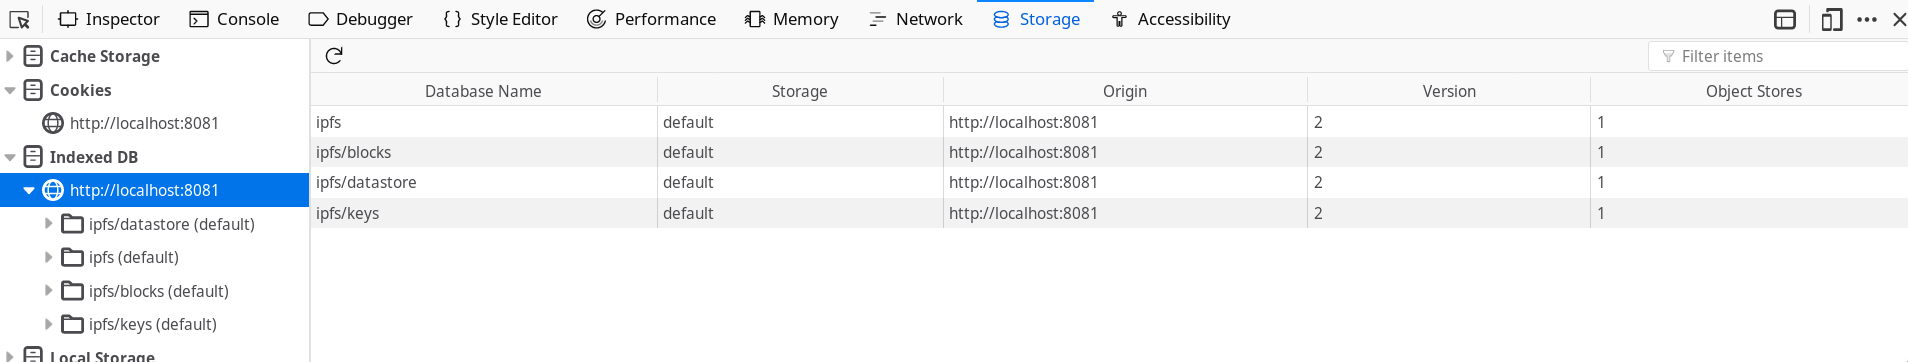
\includegraphics{../images/ipfs_browser.png}
\caption{An image showing the IPFS IndexedDB databases in Firefox}
\end{figure}
}

Note since you have not explicitly defined a database in the broser, no
IndexedDB databases have been created for OrbitDB yet.

\begin{quote}
\textbf{Caution!} iOS and Android have been known to purge IndexedDB if
storage space needs to be created inside of your phone. We recommend
creating robust backup mechanisms at the application layer.
\end{quote}

\subsection{Creating a Database}\label{creating-a-database-1}

Now, you will create a local database that \emph{only you} can read.

Inside of the \texttt{NewPiecePlease} constructor, Expand the IPFS
\texttt{ready} event handler to the following, and then run the code:

\begin{Shaded}
\begin{Highlighting}[]
\VariableTok{node}\NormalTok{.}\AttributeTok{on}\NormalTok{(}\StringTok{"ready"}\OperatorTok{,} \AttributeTok{async}\NormalTok{ () }\OperatorTok{=>} \OperatorTok{\{}
\NormalTok{  orbitdb }\OperatorTok{=}\NormalTok{ await }\VariableTok{OrbitDB}\NormalTok{.}\AttributeTok{createInstance}\NormalTok{(node)}

  \KeywordTok{const}\NormalTok{ options }\OperatorTok{=} \OperatorTok{\{}
    \DataTypeTok{accessController}\OperatorTok{:} \OperatorTok{\{} \DataTypeTok{write}\OperatorTok{:}\NormalTok{ [}\VariableTok{orbitdb}\NormalTok{.}\VariableTok{identity}\NormalTok{.}\AttributeTok{publicKey}\NormalTok{] }\OperatorTok{\},}
    \DataTypeTok{indexBy}\OperatorTok{:} \StringTok{"hash"}
  \OperatorTok{\}}
  
\NormalTok{  piecesDb }\OperatorTok{=}\NormalTok{ await }\VariableTok{orbitdb}\NormalTok{.}\AttributeTok{docstore}\NormalTok{(}\StringTok{'pieces'}\OperatorTok{,}\NormalTok{ options)}
  \VariableTok{console}\NormalTok{.}\AttributeTok{log}\NormalTok{(}\VariableTok{piecesDb}\NormalTok{.}\AttributeTok{id}\NormalTok{)}
\OperatorTok{\}}\NormalTok{)}
\end{Highlighting}
\end{Shaded}

You will see something like the following as an output:
\texttt{/orbitdb/zdpuB3VvBJHqYCocN4utQrpBseHou88mq2DLh7bUkWviBQSE3/pieces}.
This is the id, or \textbf{address} (technically a multiaddress) of this
database. It's important for you to not only \emph{know} this, but also
to understand what it is.

The first bit, \texttt{/orbitdb}, is the protocol. It tells you that
this address is an OrbitDB address. The last bit, \texttt{pieces} is
simply the name you provided.

It's the second, or middle, part
\texttt{zdpuB3VvBJHqYCocN4utQrpBseHou88mq2DLh7bUkWviBQSE3} that is the
most interesting. This value comes from the combining three pieces of
data, and then hashing them: 1. The \textbf{access control list} of the
database 2. The \textbf{type} of the database 3. The \textbf{name} of
the database

\begin{quote}
\emph{Note:} Misunderstanding OrbitDB addressing can lead to some very
unexpected - sometimes hilarious, sometimes disastrous outcomes. Read
more in Part 2 to learn more.
\end{quote}

\subsubsection{What just happened?}\label{what-just-happened-4}

Your code created a local OrbitDB database, of type ``docstore'',
writable only by you.

\begin{itemize}
\tightlist
\item
  The \texttt{options} defines the paramaters for the database we are
  about to create.
\item
  \texttt{accessController:\ \{\ write:\ {[}orbitdb.identity.publicKey{]}\ \}}
  defines the ACL, or ``Access Control List''. In this instance we are
  restricting \texttt{write} access to ONLY orbitdb instances identified
  by our particular \texttt{publicKey}
\item
  \texttt{indexBy:\ "hash"} is a docstore-specific option, which
  specifies which field to index our database by
\item
  \texttt{pieces\ =\ await\ orbitdb.docstore(\textquotesingle{}pieces\textquotesingle{},\ options)}
  is the magic line that creates the database. Once this line is
  completed, the database is open and can be acted upon.
\end{itemize}

\begin{quote}
\textbf{Caution!} A note about identity: Your public key is not your
identity. We repeat, \emph{your public key is not your identity}.
Though, it is often used as such for convenience's sake, and the lack of
better alternatives. So, in the early parts of this tutorial we say
``writable only to you'' when we really mean ``writable only by an
OrbitDB instance on top of an IPFS node that has the correct id, which
we are assuming is controlled by you.''
\end{quote}

See for more info:
https://github.com/orbitdb/orbit-db/blob/525978e0a916a8b027e9ea73d8736acb2f0bc6b4/src/OrbitDB.js\#L106

\paragraph{What else happened in
node.js?}\label{what-else-happened-in-node.js-3}

You will see some activity inside your project's \texttt{orbitdb/}
folder. This is good.

\begin{Shaded}
\begin{Highlighting}[]
\NormalTok{$ }\FunctionTok{ls}\NormalTok{ orbitdb/}
\ExtensionTok{QmNrPunxswb2Chmv295GeCvK9FDusWaTr1ZrYhvWV9AtGM/}\NormalTok{  zdpuB3VvBJHqYCocN4utQrpBseHou88mq2DLh7bUkWviBQSE3/}

\NormalTok{$ }\FunctionTok{ls}\NormalTok{ orbitdb/zdpuB3VvBJHqYCocN4utQrpBseHou88mq2DLh7bUkWviBQSE3/}
\ExtensionTok{pieces/}

\NormalTok{$ }\FunctionTok{ls}\NormalTok{ orbitdb/zdpuB3VvBJHqYCocN4utQrpBseHou88mq2DLh7bUkWviBQSE3/pieces/}
\ExtensionTok{000003.log}\NormalTok{  CURRENT  LOCK  LOG  MANIFEST-000002}
\end{Highlighting}
\end{Shaded}

You don't need to understand this fully for now, just know that it
happened. Two subfolders, one being the original folder you saw when you
instantiated OrbitDB, and now another that has the same address as your
database.

\paragraph{What else happened in the
browser?}\label{what-else-happened-in-the-browser-3}

Similarly, a new IndexedDB database was created to hold your
OrbitDB-specific info, apart from the data itself which are still stored
in IPFS.

\hypertarget{}{
\begin{figure}
\centering
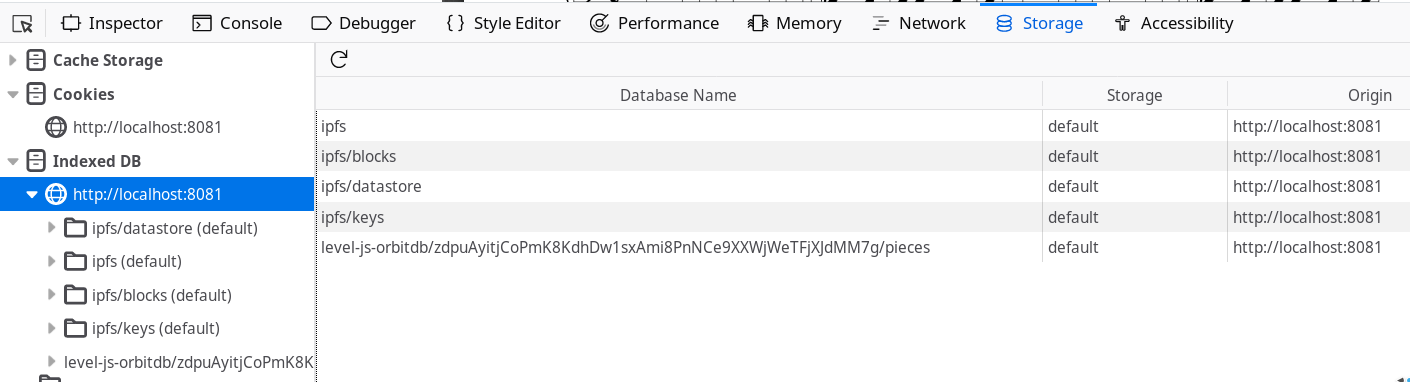
\includegraphics{../images/ipfs_browser_2.png}
\caption{An image showing the IPFS and OrbitDB IndexedDB databases in
Firefox}
\end{figure}
}

This shows you one of OrbitDB's core strenths - the ability to manage a
lot of complexity between its own internals and tht of IPFS, providing a
clear and clean API to manage the data that matters to you.

\hypertarget{choosing-a-data-store}{\subsection{Choosing a data
store}\label{choosing-a-data-store}}

OrbitDB organizes its functionality by separating different data
management concerns, schemas and APIs into \textbf{stores}. We chose a
\texttt{docstore} for you in the last chapter, but after this tutorial
it will be your job to determine the right store for the job.

At your disposal you have:

\begin{itemize}
\tightlist
\item
  \textbf{\href{https://github.com/orbitdb/orbit-db/blob/master/API.md\#orbitdblognameaddress}{log}}:
  an immutable (append-only) log with traversable history. Useful for
  \emph{``latest N''} use cases or as a message queue.
\item
  \textbf{\href{https://github.com/orbitdb/orbit-db/blob/master/API.md\#orbitdbfeednameaddress}{feed}}:
  a mutable log with traversable history. Entries can be added and
  removed. Useful for \emph{``shopping cart''} type of use cases, or for
  example as a feed of blog posts or ``tweets''.
\item
  \textbf{\href{https://github.com/orbitdb/orbit-db/blob/master/API.md\#orbitdbkeyvaluenameaddress}{keyvalue}}:
  a key-value database just like your favourite key-value database.
\item
  \textbf{\href{https://github.com/orbitdb/orbit-db/blob/master/API.md\#orbitdbdocsnameaddress-options}{docs}}:
  a document database to which JSON documents can be stored and indexed
  by a specified key. Useful for building search indices or version
  controlling documents and data.
\item
  \textbf{\href{https://github.com/orbitdb/orbit-db/blob/master/API.md\#orbitdbcounternameaddress}{counter}}:
  Useful for counting events separate from log/feed data.
\end{itemize}

Each OrbitDB store has its own specific API methods to create, delete,
retreieve and update data. In general, you can expect to always have
something like a \texttt{get} and something like a \texttt{put}.

Also, users of OrbitDB can write their own stores if it suits them. This
is an advanced topic and is covered in Part 3 of this book.

\hypertarget{key-takeaways}{\subsection{Key
Takeaways}\label{key-takeaways}}

\begin{itemize}
\tightlist
\item
  OrbitDB is a distributed database layer which stores its raw data in
  IPFS
\item
  Both IPFS and OrbitDB work offline and online
\item
  OrbitDB instances have an \emph{ID} which is the same as the underling
  IPFS node's ID.
\item
  OrbitDB instances create databases, which have unique \emph{addresses}
\item
  Basic access rights to OrbitDB databases are managed using access
  control lists (or ACLs), based on the ID of the IPFS node performing
  the requests on the database
\item
  OrbitDB database addresses are hashes of the database's ACL, its type,
  and its name.
\item
  Since OrbitDB and IPFS are written in JavaScript, it is possible to
  build isomorphic applications that run in the browser and in node.js
\item
  OrbitDB manages needed flexibility of schema and API design in
  functionality called \textbf{stores}.
\item
  OrbitDB comes with a handful of stores, and you can write your own.
\item
  Each store will have its own API, but you will generally have at least
  a \texttt{get} and a \texttt{put}
\end{itemize}

Now that you've laid the groudnwork, you'll learn how to work with data!
Onward, then, to \href{./02_Managing_Data.md}{Chapter 2: Managing Data}.

\begin{itemize}
\tightlist
\item
  Resolves \#\href{https://github.com/orbitdb/orbit-db/issues/367}{367}
\item
  Resolves \#\href{https://github.com/orbitdb/orbit-db/issues/366}{366}
\item
  Resolves \#\href{https://github.com/orbitdb/orbit-db/issues/502}{502}
\end{itemize}

\textbf{Note:} Please complete \href{./01_Basics.md}{Chapter 1 - Laying
the Foundation} first.

\section{Chapter 2 - Managing Data}\label{chapter-2---managing-data}

\begin{quote}
Managing data in OrbitDB involves \emph{loading databases into memory},
and then \emph{creating}, \emph{updating}, \emph{reading}, and
\emph{deleting data}.
\end{quote}

\begin{itemize}
\tightlist
\item
  \protect\hyperlink{loading-the-database}{Loading the database}
\item
  \protect\hyperlink{adding-data}{Adding data}
\item
  \protect\hyperlink{reading-data}{Reading data}
\item
  \protect\hyperlink{updating-and-deleting-data}{Updating and deleting
  data}
\item
  \protect\hyperlink{storing-media-files}{Storing media files}
\item
  \protect\hyperlink{key-takeaways}{Key Takeaways}
\end{itemize}

\hypertarget{loading-the-database}{\subsection{Loading the
database}\label{loading-the-database}}

To start, you'll do a couple of things to enhance our current code and
tidy up. We will also scaffold out some functions to be filled in later.

Update your \texttt{NewPiecePlease\ class} handler, adding \textbf{one
line} at the bottom of the IPFS \texttt{ready} handler. and then run
this code:

\begin{Shaded}
\begin{Highlighting}[]
\KeywordTok{class}\NormalTok{ NewPiecePlease }\OperatorTok{\{}
  \AttributeTok{constructor}\NormalTok{ (IPFS}\OperatorTok{,}\NormalTok{ OrbitDB) }\OperatorTok{\{}
    \KeywordTok{this}\NormalTok{.}\AttributeTok{node} \OperatorTok{=} \KeywordTok{new} \AttributeTok{IPFS}\NormalTok{(}\OperatorTok{\{}
      \DataTypeTok{preload}\OperatorTok{:} \OperatorTok{\{} \DataTypeTok{enabled}\OperatorTok{:} \KeywordTok{false} \OperatorTok{\},}
      \DataTypeTok{EXPERIMENTAL}\OperatorTok{:} \OperatorTok{\{} \DataTypeTok{pubsub}\OperatorTok{:} \KeywordTok{true} \OperatorTok{\},}
      \DataTypeTok{repo}\OperatorTok{:} \StringTok{"./ipfs"}\OperatorTok{,}
      \DataTypeTok{config}\OperatorTok{:} \OperatorTok{\{} 
        \DataTypeTok{Bootstrap}\OperatorTok{:}\NormalTok{ []}\OperatorTok{,}
        \DataTypeTok{Addresses}\OperatorTok{:} \OperatorTok{\{} \DataTypeTok{Swarm}\OperatorTok{:}\NormalTok{ [] }\OperatorTok{\}}
      \OperatorTok{\}}
    \OperatorTok{\}}\NormalTok{)}\OperatorTok{;}

    \KeywordTok{this}\NormalTok{.}\VariableTok{node}\NormalTok{.}\AttributeTok{on}\NormalTok{(}\StringTok{"error"}\OperatorTok{,}\NormalTok{ (e) }\OperatorTok{=>} \VariableTok{console}\NormalTok{.}\AttributeTok{error}\NormalTok{)}
    \KeywordTok{this}\NormalTok{.}\VariableTok{node}\NormalTok{.}\AttributeTok{on}\NormalTok{(}\StringTok{"ready"}\OperatorTok{,} \AttributeTok{async}\NormalTok{ () }\OperatorTok{=>} \OperatorTok{\{}
      \KeywordTok{this}\NormalTok{.}\AttributeTok{orbitdb} \OperatorTok{=}\NormalTok{ await }\VariableTok{OrbitDB}\NormalTok{.}\AttributeTok{createInstance}\NormalTok{(}\KeywordTok{this}\NormalTok{.}\AttributeTok{node}\NormalTok{)}

      \KeywordTok{const}\NormalTok{ options }\OperatorTok{=} \OperatorTok{\{}
        \DataTypeTok{accessController}\OperatorTok{:} \OperatorTok{\{} \DataTypeTok{write}\OperatorTok{:}\NormalTok{ [}\KeywordTok{this}\NormalTok{.}\VariableTok{orbitdb}\NormalTok{.}\VariableTok{identity}\NormalTok{.}\AttributeTok{publicKey}\NormalTok{] }\OperatorTok{\},}
        \DataTypeTok{indexBy}\OperatorTok{:} \StringTok{'hash'}
      \OperatorTok{\}}

      \KeywordTok{this}\NormalTok{.}\AttributeTok{piecesDb} \OperatorTok{=}\NormalTok{ await }\KeywordTok{this}\NormalTok{.}\VariableTok{orbitdb}\NormalTok{.}\AttributeTok{docstore}\NormalTok{(}\StringTok{'pieces'}\OperatorTok{,}\NormalTok{ options)}
\NormalTok{      await }\KeywordTok{this}\NormalTok{.}\VariableTok{piecesDb}\NormalTok{.}\AttributeTok{load}\NormalTok{()  }\CommentTok{// It's only this line that changed!! Blink and you'll miss it}
    \OperatorTok{\}}\NormalTok{)}\OperatorTok{;}
  \OperatorTok{\}}

\NormalTok{  async }\AttributeTok{addNewPiece}\NormalTok{() }\OperatorTok{\{} \OperatorTok{\}}
\NormalTok{  async }\AttributeTok{deletePieceByHash}\NormalTok{() }\OperatorTok{\{} \OperatorTok{\}}
  \AttributeTok{getAllPieces}\NormalTok{() }\OperatorTok{\{\}}
  \AttributeTok{getPiecesByInstrument}\NormalTok{() }\OperatorTok{\{} \OperatorTok{\}}
  \AttributeTok{getPieceByHash}\NormalTok{() }\OperatorTok{\{} \OperatorTok{\}}
\NormalTok{  await }\AttributeTok{updatePieceByHash}\NormalTok{()}
\OperatorTok{\}}
\end{Highlighting}
\end{Shaded}

\subsubsection{What just happened?}\label{what-just-happened-5}

After you instantiated the database, you loaded its contents into memory
for use. It's empty for now, but not for long! Loading the database at
this point after instantiation will save you trouble later.

\begin{itemize}
\tightlist
\item
  \texttt{await\ piecesDb.load()} is a function that will need to be
  called whenever we want the latest and greatest snapshot of data in
  the database. \texttt{load()} retrieves all of the values via their
  \emph{content addresses} and loads the content into memory
\end{itemize}

\begin{quote}
\textbf{Note:} You're probably wondering about if you have a large
database of millions of documents, and the implications of loading them
all into memory. It's a valid concern, and you should move on to Part 4
of this book once you're done with the tutorial.
\end{quote}

\hypertarget{adding-data}{\subsection{Adding data}\label{adding-data}}

Now that you have a database set up, adding content to it is fairly
easy. Run the following code to add some sheet music to the repository.

We have uploaded and pinned a few piano scores to IPFS, and will provide
the hashes. You can add these hashes to your database by fleshing out
and using the \texttt{addNewPiece} function.

\begin{quote}
\textbf{Note:} We hope you like the original Metroid game, or at least
the music from it!
\end{quote}

\begin{Shaded}
\begin{Highlighting}[]
\NormalTok{async }\AttributeTok{addNewPiece}\NormalTok{(hash}\OperatorTok{,}\NormalTok{ instrument }\OperatorTok{=} \StringTok{"Piano"}\NormalTok{) }\OperatorTok{\{}
  \KeywordTok{const}\NormalTok{ cid }\OperatorTok{=}\NormalTok{ await }\VariableTok{piecesDb}\NormalTok{.}\AttributeTok{put}\NormalTok{(}\OperatorTok{\{}\NormalTok{ hash}\OperatorTok{,}\NormalTok{ instrument }\OperatorTok{\}}\NormalTok{)}
  \ControlFlowTok{return}\NormalTok{ cid}
\OperatorTok{\}}
\end{Highlighting}
\end{Shaded}

Then, in your application code, node.js or browser, you cna use this
function like so, utilizing the detault value for the
\texttt{instrument} argument.

\begin{Shaded}
\begin{Highlighting}[]
\KeywordTok{const}\NormalTok{ cid }\OperatorTok{=} \VariableTok{NPP}\NormalTok{.}\AttributeTok{addNewPiece}\NormalTok{(}\StringTok{"QmNR2n4zywCV61MeMLB6JwPueAPqheqpfiA4fLPMxouEmQ"}\NormalTok{)}
\KeywordTok{const}\NormalTok{ content }\OperatorTok{=}\NormalTok{ await }\VariableTok{NPP}\NormalTok{.}\VariableTok{node}\NormalTok{.}\VariableTok{dag}\NormalTok{.}\AttributeTok{get}\NormalTok{(cid)}
\VariableTok{console}\NormalTok{.}\AttributeTok{log}\NormalTok{(}\VariableTok{content}\NormalTok{.}\VariableTok{value}\NormalTok{.}\AttributeTok{payload}\NormalTok{)}
\end{Highlighting}
\end{Shaded}

Running this code should give you something like the following output.
Hold steady, it's overwhelming but it will make sense after we explain
what happened. For more information see Part 3.

\begin{Shaded}
\begin{Highlighting}[]
\FunctionTok{\{}
  \DataTypeTok{"op"}\FunctionTok{:}\StringTok{"PUT"}\FunctionTok{,}
  \DataTypeTok{"key"}\FunctionTok{:}\StringTok{"QmNR2n4zywCV61MeMLB6JwPueAPqheqpfiA4fLPMxouEmQ"}\FunctionTok{,}
  \DataTypeTok{"value"}\FunctionTok{:} \FunctionTok{\{}
    \DataTypeTok{"hash"}\FunctionTok{:}\StringTok{"QmNR2n4zywCV61MeMLB6JwPueAPqheqpfiA4fLPMxouEmQ"}\FunctionTok{,}
    \DataTypeTok{"instrument"}\FunctionTok{:}\StringTok{"Accordion"}
  \FunctionTok{\}}
\FunctionTok{\}}
\end{Highlighting}
\end{Shaded}

\subsubsection{What just happened?}\label{what-just-happened-6}

\begin{itemize}
\tightlist
\item
  \texttt{piecesDb.put(\{\ ...\ \})} is the most important line here.
  This call takes an object to sture and returns a \emph{mutlihash},
  which is the hash of the content added to IPFS.
\item
  \texttt{node.dag.get(hash)} is a function that takes a Content ID
  (CID) and returns content.
\item
  \texttt{"op":\ "PUT"}is a notable part of the output. At the core of
  OrbitDB databases is the \textbf{OPLOG}, where all data are stored as
  a log of operations, which are then calculated into the appropriate
  schema for application use. The operation is specified here as a
  \texttt{PUT}, and then the \texttt{key}/\texttt{value} pair is your
  data.
\end{itemize}

\begin{quote}
\textbf{Note:} ``dag'' in the code refers to the acronym DAG, which
stands for Directed Acyclic Graph. This is a data structure that is, or
is at least closely related to Blockchain. More on this in Part 4
\end{quote}

You can repeat this process to add more hashes from the NES Metroid
soundtrack:

\begin{verbatim}
QmNR2n4zywCV61MeMLB6JwPueAPqheqpfiA4fLPMxouEmQ | Metroid - Ending Theme.pdf
QmRn99VSCVdC693F6H4zeS7Dz3UmaiBiSYDf6zCEYrWynq | Metroid - Escape Theme.pdf
QmdzDacgJ9EQF9Z8G3L1fzFwiEu255Nm5WiCey9ntrDPSL | Metroid - Game Start.pdf
QmcFUvG75QTMok9jrteJzBUXeoamJsuRseNuDRupDhFwA2 | Metroid - Item Found.pdf
QmTjszMGLb5gKWAhFZbo8b5LbhCGJkgS8SeeEYq3P54Vih | Metroid - Kraids Hideout.pdf
QmNfQhx3WvJRLMnKP5SucMRXEPy9YQ3V1q9dDWNC6QYMS3 | Metroid - Norfair.pdf
QmQS4QNi8DCceGzKjfmbBhLTRExNboQ8opUd988SLEtZpW | Metroid - Ridleys Hideout.pdf
QmcJPfExkBAZe8AVGfYHR7Wx4EW1Btjd5MXX8EnHCkrq54 | Metroid - Silence.pdf
Qmb1iNM1cXW6e11srUvS9iBiGX4Aw5dycGGGDPTobYfFBr | Metroid - Title Theme.pdf
QmYPpj6XVNPPYgwvN4iVaxZLHy982TPkSAxBf2rzGHDach | Metroid - Tourian.pdf
QmefKrBYeL58qyVAaJoGHXXEgYgsJrxo763gRRqzYHdL6o | Metroid - Zebetite.pdf
\end{verbatim}

These are all stored in the global IPFS network so you can find any
piece by visiting a public gateway such as \texttt{ipfs.io} and adding
the IPFS multiaddress to the end of the URL like so:
https://ipfs.io/ipfs/QmYPpj6XVNPPYgwvN4iVaxZLHy982TPkSAxBf2rzGHDach

\hypertarget{reading-data}{\subsection{Reading
data}\label{reading-data}}

You've added data to your local database, and now you'll can query it.
OrbitDB gives you a number of ways to do this, mostly based on which
\emph{store} you picked.

We gave you a \texttt{docstore} earlier, so you can flesh out the all of
thet simple \texttt{get*****} functions like so. \texttt{docstore} also
provides the more puwerful \texttt{query} function, which we can
abstract to write a \texttt{getPiecesByInstrument} function:

\begin{Shaded}
\begin{Highlighting}[]
\AttributeTok{getAllPieces}\NormalTok{() }\OperatorTok{\{}
  \KeywordTok{const}\NormalTok{ pieces }\OperatorTok{=} \KeywordTok{this}\NormalTok{.}\VariableTok{piecesDb}\NormalTok{.}\AttributeTok{get}\NormalTok{(}\StringTok{''}\NormalTok{)}
  \ControlFlowTok{return}\NormalTok{ pieces}
\OperatorTok{\}}

\AttributeTok{getPieceByHash}\NormalTok{(hash) }\OperatorTok{\{}
  \KeywordTok{const}\NormalTok{ singlePiece }\OperatorTok{=} \KeywordTok{this}\NormalTok{.}\VariableTok{piecesDb}\NormalTok{.}\AttributeTok{get}\NormalTok{(hash)[}\DecValTok{0}\NormalTok{]}
  \ControlFlowTok{return}\NormalTok{ singlePiece}
\OperatorTok{\}}

\AttributeTok{getByInstrument}\NormalTok{(instrument) }\OperatorTok{\{}
  \ControlFlowTok{return} \KeywordTok{this}\NormalTok{.}\VariableTok{piecesDb}\NormalTok{.}\AttributeTok{query}\NormalTok{((piece) }\OperatorTok{=>} \VariableTok{piece}\NormalTok{.}\AttributeTok{instrument} \OperatorTok{===}\NormalTok{ instrument)}
\OperatorTok{\}}
\end{Highlighting}
\end{Shaded}

In your application code, you can use these functions it like so:

\begin{Shaded}
\begin{Highlighting}[]
\NormalTok{pieces }\OperatorTok{=} \VariableTok{NPP}\NormalTok{.}\AttributeTok{getAllPieces}\NormalTok{()}
\VariableTok{pleces}\NormalTok{.}\AttributeTok{forEach}\NormalTok{((piece) }\OperatorTok{=>} \OperatorTok{\{} \CommentTok{/* do something */} \OperatorTok{\}}\NormalTok{)}

\NormalTok{piece }\OperatorTok{=} \VariableTok{NPP}\NormalTok{.}\AttributeTok{getPieceByHash}\NormalTok{(}\StringTok{'QmNR2n4zywCV61MeMLB6JwPueAPqheqpfiA4fLPMxouEmQ'}\NormalTok{)}
\VariableTok{console}\NormalTok{.}\AttributeTok{log}\NormalTok{(piece)}
\end{Highlighting}
\end{Shaded}

Pulling a random score from the database is a great way to find random
music to practice. Run this code:

\begin{Shaded}
\begin{Highlighting}[]
\KeywordTok{const}\NormalTok{ pieces }\OperatorTok{=} \VariableTok{NPP}\NormalTok{.}\AttributeTok{getPieceByInstrument}\NormalTok{(}\StringTok{"Piano"}\NormalTok{)}
\KeywordTok{const}\NormalTok{ randomPiece }\OperatorTok{=}\NormalTok{ pieces[}\VariableTok{items}\NormalTok{.}\AttributeTok{length} \OperatorTok{*} \VariableTok{Math}\NormalTok{.}\AttributeTok{random}\NormalTok{() }\OperatorTok{|} \DecValTok{0}\NormalTok{]}
\VariableTok{console}\NormalTok{.}\AttributeTok{log}\NormalTok{(randomPiece)}
\end{Highlighting}
\end{Shaded}

Both \texttt{console.log} calls above will return something like this.

\begin{Shaded}
\begin{Highlighting}[]
\FunctionTok{\{}
  \DataTypeTok{"hash"}\FunctionTok{:}\StringTok{"QmNR2n4zywCV61MeMLB6JwPueAPqheqpfiA4fLPMxouEmQ"}\FunctionTok{,}
  \DataTypeTok{"instrument"}\FunctionTok{:}\StringTok{"Accordion"}
\FunctionTok{\}}
\end{Highlighting}
\end{Shaded}

\subsubsection{What just happened?}\label{what-just-happened-7}

You queried the database of scores you created earlier in the chapter,
retrieving by hash and also randomly.

\begin{itemize}
\tightlist
\item
  \texttt{pieces.get(hash)} is a simple function that performs a partial
  string search on your database indexes. It will return an array of
  records that match. As you can see in your \texttt{getAllPieces}
  function, you can pass an empty string to return all pieces.
\item
  \texttt{return\ this.piecesDb.query((piece)\ =\textgreater{}\ piece.instrument\ ===\ instrument)}
  queries the database, returning. It's most analagous to JavaScripts
  \texttt{Array.filter} method.
\end{itemize}

\begin{quote}
\textbf{Note:} Generally speaking, \texttt{get} functions do not return
promises since the calculation of database state happens at the time of
a \emph{write}. This is a trade-off to allow for ease of use and
performance based on the assumption that writes are \emph{generally}
less frequent than reads.
\end{quote}

\hypertarget{updating-and-deleting-data}{\subsection{Updating and
deleting data}\label{updating-and-deleting-data}}

You'll next want to provide your users with the ability to update and
delete their pieces. For example if you realize you'd rather practice a
piece on a harpsichord instead of a piano, or if they want to stop
practicing a certain piece.

Again, each OrbitDB store may have slightly different methods for this.
In the \texttt{docstore} you can update records by again using the
\texttt{put} method and the ID of the index you want to update.

\begin{Shaded}
\begin{Highlighting}[]
\NormalTok{async }\AttributeTok{updatePieceByHash}\NormalTok{(hash}\OperatorTok{,}\NormalTok{ instrument }\OperatorTok{=} \StringTok{"Piano"}\NormalTok{) }\OperatorTok{\{}
  \KeywordTok{var}\NormalTok{ piece }\OperatorTok{=}\NormalTok{ await }\KeywordTok{this}\NormalTok{.}\AttributeTok{getPieceByHash}\NormalTok{(hash)}
  \VariableTok{piece}\NormalTok{.}\AttributeTok{instrument} \OperatorTok{=}\NormalTok{ instrument}
  \KeywordTok{const}\NormalTok{ cid }\OperatorTok{=}\NormalTok{ await }\KeywordTok{this}\NormalTok{.}\VariableTok{piecesDb}\NormalTok{.}\AttributeTok{put}\NormalTok{(piece)}
  \ControlFlowTok{return}\NormalTok{ cid}
\OperatorTok{\}}
\end{Highlighting}
\end{Shaded}

Deleting a record by hash is also easy:

\begin{Shaded}
\begin{Highlighting}[]
\NormalTok{async }\AttributeTok{deletePieceByHash}\NormalTok{(hash) }\OperatorTok{\{}
  \KeywordTok{const}\NormalTok{ cid }\OperatorTok{=}\NormalTok{ await }\KeywordTok{this}\NormalTok{.}\VariableTok{piecesDb}\NormalTok{.}\AttributeTok{del}\NormalTok{(hash)}
  \ControlFlowTok{return}\NormalTok{ cid}
\OperatorTok{\}}
\end{Highlighting}
\end{Shaded}

In your application code, you can run these new functions and see the
opcodes that return to get a sense of what's going on.

\begin{Shaded}
\begin{Highlighting}[]
\KeywordTok{const}\NormalTok{ cid }\OperatorTok{=}\NormalTok{ await }\VariableTok{NPP}\NormalTok{.}\AttributeTok{updatePiece}\NormalTok{(}\StringTok{"QmNR2n4zywCV61MeMLB6JwPueAPqheqpfiA4fLPMxouEmQ"}\OperatorTok{,} \StringTok{"Harpsichord"}\NormalTok{)}
\CommentTok{// do stuff with the cid as above}

\KeywordTok{const}\NormalTok{ cid }\OperatorTok{=}\NormalTok{ await }\VariableTok{NPP}\NormalTok{.}\AttributeTok{deletePieceByHash}\NormalTok{(}\StringTok{"QmNR2n4zywCV61MeMLB6JwPueAPqheqpfiA4fLPMxouEmQ"}\NormalTok{)}
\KeywordTok{const}\NormalTok{ content }\OperatorTok{=}\NormalTok{ await }\VariableTok{NPP}\NormalTok{.}\VariableTok{node}\NormalTok{.}\VariableTok{dag}\NormalTok{.}\AttributeTok{get}\NormalTok{(cid)}
\VariableTok{console}\NormalTok{.}\AttributeTok{log}\NormalTok{(}\VariableTok{content}\NormalTok{.}\VariableTok{value}\NormalTok{.}\AttributeTok{payload}\NormalTok{)}
\end{Highlighting}
\end{Shaded}

While the opcode for PUT will be the same, the opcode for
\texttt{deletePieceByHash} is not:

\begin{Shaded}
\begin{Highlighting}[]
\FunctionTok{\{}
  \DataTypeTok{"op"}\FunctionTok{:}\StringTok{"DEL"}\FunctionTok{,}
  \DataTypeTok{"key"}\FunctionTok{:}\StringTok{"QmdzDacgJ9EQF9Z8G3L1fzFwiEu255Nm5WiCey9ntrDPSL"}\FunctionTok{,}
  \DataTypeTok{"value"}\FunctionTok{:}\KeywordTok{null}
\FunctionTok{\}}
\end{Highlighting}
\end{Shaded}

\subsubsection{What just happened?}\label{what-just-happened-8}

You may be thinking something like this: ``Wait, if OrbitDB is built
upon IPFS and IPFS is immutable, then how are we updating or deleting
records?'' Great question, and the answer lies in the opcodes Let's step
through the code so we can get to that.

\begin{itemize}
\tightlist
\item
  \texttt{this.piecesDb.put} is nothing new, we're just using it to
  perform an update instead of an insert
\item
  \texttt{this.piecesDb.del} is a simple function that takes a hash,
  deletes the record, and returns a CID
\item
  \texttt{"op":\ "DEL"} is another opcode, \texttt{DEL} for DELETE. This
  log entry effectively removes this key from your records and also
  removes the content from your local IPFS
\end{itemize}

\hypertarget{storing-media-files}{\subsection{Storing Media
Files}\label{storing-media-files}}

We are often asked if it is possible to store media files like pictures
or audio directly inside OrbitDB. Our answer is that you should treat
this like any other database system and store the \emph{address} of the

Luckily, with content addressing in IPFS, this becomes rather easy, and
predictable from a schema design standpoint. The overall pattern in:

\begin{enumerate}
\def\labelenumi{\arabic{enumi}.}
\tightlist
\item
  Add the file to IPFS, which will return the \emph{multihash} of the
  file
\item
  Store said multihash in OrbitDB
\item
  When it comes time to display the media, use native IPFS functionality
  to retrieve it from the hash
\end{enumerate}

To see this in action,
\href{https://ipfs.io/ipfs/QmYPpj6XVNPPYgwvN4iVaxZLHy982TPkSAxBf2rzGHDach}{download
the ``Tourian'' PDF} to your local file system for use in the next
examples

\paragraph{On the command line with the go-ipfs or js-ipfs
daemon}\label{on-the-command-line-with-the-go-ipfs-or-js-ipfs-daemon}

After following the installation instructions to install
\href{}{go-ipfs} or \href{}{js-ipfs} globally, you can run the following
command:

\begin{Shaded}
\begin{Highlighting}[]
\NormalTok{$ }\ExtensionTok{ipfs}\NormalTok{ add file.pdf}
\ExtensionTok{QmYPpj6XVNPPYgwvN4iVaxZLHy982TPkSAxBf2rzGHDach}
\end{Highlighting}
\end{Shaded}

You can then use that hash in the same manner as above to add it to the
database of pieces.

\paragraph{In Node.js}\label{in-node.js-1}

In Node.JS, adding a file from the filesystem can be accomplished like
so:

\begin{Shaded}
\begin{Highlighting}[]
\KeywordTok{var}\NormalTok{ IPFS }\OperatorTok{=} \AttributeTok{require}\NormalTok{(}\StringTok{'ipfs'}\NormalTok{)}
\KeywordTok{var}\NormalTok{ ipfs }\OperatorTok{=} \KeywordTok{new} \AttributeTok{IPFS}\NormalTok{(}\CommentTok{/* insert appropriate options here for your local IPFS installation */}\NormalTok{)}

\VariableTok{ipfs}\NormalTok{.}\AttributeTok{addFromFs}\NormalTok{(}\StringTok{"./file.pdf"}\NormalTok{).}\AttributeTok{then}\NormalTok{(}\VariableTok{console}\NormalTok{.}\AttributeTok{log}\NormalTok{)}
\end{Highlighting}
\end{Shaded}

\paragraph{In the browser}\label{in-the-browser-1}

Unfortunately we don't have a one-line trick to upload a file to IPFS,
but if you have a HTML file input with an ID of ``fileUpload'', you can
do the following:

\begin{Shaded}
\begin{Highlighting}[]
\KeywordTok{var}\NormalTok{ fileInput }\OperatorTok{=} \VariableTok{document}\NormalTok{.}\AttributeTok{getElementById}\NormalTok{(}\StringTok{"fileUpload"}\NormalTok{)}
\end{Highlighting}
\end{Shaded}

\subsubsection{What just happened?}\label{what-just-happened-9}

You added some potentially very large media files to IPFS, and then
stored the 40-byte addresses in OrbitDB for retrieval and use. You are
now able to leverage the benefits of both IPFS and

\begin{quote}
\textbf{Note:} IPFS nodes run \emph{inside} the browser, so if you're
adding lots of files via the above method, keep an eye on your IndexedDB
usage, since that's where IPFS is storing the blocks.
\end{quote}

\subsection{Key Takeaways}\label{key-takeaways-1}

\begin{itemize}
\tightlist
\item
  Calling \texttt{load()} periodically ensures you have the latest
  entries from the database
\item
  Generally speaking, a \texttt{put} or \texttt{delete} will return a
  Promise (or require \texttt{await}), and a \texttt{get} will return
  the value(s) immediately.
\item
  Updating the database is equivalent to adding a new entry to its
  OPLOG.
\item
  The OPLOG is calculated to give the current \emph{state} of the
  database, which is the view you generally interact with
\item
  OPLOGS are flexible, particularly if you're writing your own stores.
  \texttt{docstore} primarily utilizes the \texttt{PUT} and \texttt{DEL}
  opcodes
\item
  While you technically \emph{can} store encoded media directly in a
  database, media files are best stored in OrbitDB as IPFS hashes
\item
  Keep an eye on IndexedDB size and limitations when adding content to
  IPFS via the browser.
\end{itemize}

Of course, in the vast majority of apps you create, you won't just be
interacting with one database or one type of data. We've got you covered
in \href{03_Structuring_Data.md}{Chapter 3: Structuring Data}

\begin{itemize}
\tightlist
\item
  Resolves \#\href{https://github.com/orbitdb/orbit-db/issues/365}{365}
\item
  Resolves \#\href{https://github.com/orbitdb/orbit-db/issues/438}{438}
\item
  Resolves \#\href{https://github.com/orbitdb/orbit-db/issues/381}{381}
\item
  Resolves \#\href{https://github.com/orbitdb/orbit-db/issues/242}{242}
\item
  Resolves \#\href{https://github.com/orbitdb/orbit-db/issues/430}{430}
  \textbf{Note:} Please complete \href{./02_Managing_Data.md}{Chapter 2
  - Managing Data} first.
\end{itemize}

\section{Chapter 3 - Structuring your
data}\label{chapter-3---structuring-your-data}

\begin{quote}
or, ``How you learned to stop worrying and love \emph{nested
databases}.''
\end{quote}

\begin{itemize}
\tightlist
\item
  \protect\hyperlink{}{Adding a practice counter to each piece}
\item
  \protect\hyperlink{}{Utilizing your practice counter}
\item
  \protect\hyperlink{}{Adding a higher-level user database}
\item
  \protect\hyperlink{}{Updating your user profile}
\end{itemize}

\subsection{Adding a practice counter to each
piece}\label{adding-a-practice-counter-to-each-piece}

Your users may want to keep track of their practice, at minimum how many
times they practiced a piece. You'll enable that functionality for them
by creating a new OrbitDB \texttt{counter} store for each piece, and
creating a few new functions inside the \texttt{NewPiecePlease} class to
interact with the counters.

\begin{quote}
\textbf{Note:} The nesting approach detailed here is but one of many,
and you are free to organize your data as you see fit. This is a
powerful feature of OrbitDB and we are excited to see how people tackle
this problem in the future!
\end{quote}

Update the \texttt{addNewPiece} function to create a \texttt{counter}
store every time a new piece is added to the database. You can utilize
basic access control again to ensure that only a node with your IPFS
node's ID can write to it.

\begin{Shaded}
\begin{Highlighting}[]
\NormalTok{async }\AttributeTok{addNewPiece}\NormalTok{(hash}\OperatorTok{,}\NormalTok{ instrument }\OperatorTok{=} \StringTok{"Piano"}\NormalTok{) }\OperatorTok{\{}
  \KeywordTok{const}\NormalTok{ options }\OperatorTok{=} \OperatorTok{\{} \DataTypeTok{accessController}\OperatorTok{:} \OperatorTok{\{} \DataTypeTok{write}\OperatorTok{:}\NormalTok{ [}\KeywordTok{this}\NormalTok{.}\VariableTok{orbitdb}\NormalTok{.}\VariableTok{identity}\NormalTok{.}\AttributeTok{publicKey}\NormalTok{] }\OperatorTok{\}\}}
  \KeywordTok{const}\NormalTok{ dbName }\OperatorTok{=} \StringTok{"counter."} \OperatorTok{+} \VariableTok{hash}\NormalTok{.}\AttributeTok{substr}\NormalTok{(}\DecValTok{20}\OperatorTok{,}\DecValTok{20}\NormalTok{)}
  \KeywordTok{const}\NormalTok{ counterDb }\OperatorTok{=}\NormalTok{ await }\KeywordTok{this}\NormalTok{.}\VariableTok{orbitdb}\NormalTok{.}\AttributeTok{counter}\NormalTok{(dbName}\OperatorTok{,}\NormalTok{ options)}

  \KeywordTok{const}\NormalTok{ cid }\OperatorTok{=}\NormalTok{ await }\KeywordTok{this}\NormalTok{.}\VariableTok{piecesDb}\NormalTok{.}\AttributeTok{put}\NormalTok{(}\OperatorTok{\{}
    \DataTypeTok{hash}\OperatorTok{:}\NormalTok{ hash}\OperatorTok{,}
    \DataTypeTok{instrument}\OperatorTok{:}\NormalTok{ instrument}\OperatorTok{,}
    \DataTypeTok{counter}\OperatorTok{:} \VariableTok{counterDb}\NormalTok{.}\AttributeTok{id}
  \OperatorTok{\}}\NormalTok{)}

  \ControlFlowTok{return}\NormalTok{ cid}
\OperatorTok{\}}
\end{Highlighting}
\end{Shaded}

In your application code this would look something like this:

\begin{Shaded}
\begin{Highlighting}[]
\KeywordTok{const}\NormalTok{ cid }\OperatorTok{=}\NormalTok{ await }\VariableTok{NPP}\NormalTok{.}\AttributeTok{addNewPiece}\NormalTok{(}\StringTok{"QmdzDacgJ9EQF9Z8G3L1fzFwiEu255Nm5WiCey9ntrDPSL"}\OperatorTok{,} \StringTok{"Piano"}\NormalTok{)}
\KeywordTok{const}\NormalTok{ content }\OperatorTok{=}\NormalTok{ await }\VariableTok{NPP}\NormalTok{.}\VariableTok{node}\NormalTok{.}\VariableTok{dag}\NormalTok{.}\AttributeTok{get}\NormalTok{(cid)}
\VariableTok{console}\NormalTok{.}\AttributeTok{log}\NormalTok{(}\VariableTok{content}\NormalTok{.}\VariableTok{value}\NormalTok{.}\VariableTok{payload}\NormalTok{.}\AttributeTok{value}\NormalTok{)}
\end{Highlighting}
\end{Shaded}

Which will then output something like:

\begin{Shaded}
\begin{Highlighting}[]
\FunctionTok{\{}
  \DataTypeTok{"hash"}\FunctionTok{:}\StringTok{"QmdzDacgJ9EQF9Z8G3L1fzFwiEu255Nm5WiCey9ntrDPSL"}\FunctionTok{,}
  \DataTypeTok{"counter"}\FunctionTok{:}\StringTok{"/orbitdb/zdpuAoM3yZEwsynUgeWPfizmWz5DEFPiQSvg5gUPu9VoGhxjS/counter.fzFwiEu255Nm5WiCey9n"}\FunctionTok{,}
  \DataTypeTok{"instrument"}\FunctionTok{:}\StringTok{"Piano"}
\FunctionTok{\}}
\end{Highlighting}
\end{Shaded}

\subsubsection{What just happened?}\label{what-just-happened-10}

You changed your code to add a new database of type \texttt{counter} for
each new entry added to the database.

\begin{itemize}
\tightlist
\item
  \texttt{const\ options\ =\ \{\ accessController:\ \{\ write:\ {[}this.orbitdb.identity.publicKey{]}\ \}\}}
  should be recognizable from Chapter 1. This sets options for the db,
  namely the \texttt{accessController} to give write access only to your
  node's ID, or public key. `
\item
  \texttt{this.orbitdb.counter} creates a new counter type with
  \texttt{options} that provide a write ACL for your IPFS node
\item
  \texttt{const\ dbName\ =\ "counter."\ +\ hash.substr(20,20)} prepends
  \texttt{counter.} to the truncated database name. See the note below.
\item
  \texttt{this.piecesDb.put} is then modified to store the
  \emph{address} of this new database for later retrieval similar to the
  way you stored media addresses in a previous chapter.
\item
  \texttt{"counter":"/orbitdb/zdpuAoM3yZEwsynUgeWPfizmWz5DEFPiQSvg5gUPu9VoGhxjS/counter.fzFwiEu255Nm5WiCey9n"}
  in the output now reflects this change by storing the \emph{address}
  of the new DB for later retrieval and updating.
\end{itemize}

\begin{quote}
\textbf{Note:} There is a limit of 40 characters on the names of the
databases, and multihashes are over this limit at 46. We still need
unique names for each of the databases created to generate unique
addresses, so we trim down the hash and prepend it with
\texttt{counter.} to get around this limitation.
\end{quote}

\subsection{Utilizing the practice
counter}\label{utilizing-the-practice-counter}

Now, add a few functions to \texttt{NewPiecePlease} that utilize the
counters when necessary

\begin{Shaded}
\begin{Highlighting}[]
\NormalTok{async }\AttributeTok{getPracticeCount}\NormalTok{(piece) }\OperatorTok{\{}
  \KeywordTok{const}\NormalTok{ counter }\OperatorTok{=}\NormalTok{ await }\KeywordTok{this}\NormalTok{.}\VariableTok{orbitdb}\NormalTok{.}\AttributeTok{counter}\NormalTok{(}\VariableTok{piece}\NormalTok{.}\AttributeTok{counter}\NormalTok{)}
\NormalTok{  await }\VariableTok{counter}\NormalTok{.}\AttributeTok{load}\NormalTok{()}
  \ControlFlowTok{return} \VariableTok{counter}\NormalTok{.}\AttributeTok{value}
\OperatorTok{\}}

\NormalTok{async }\AttributeTok{incrementPracticeCounter}\NormalTok{(piece) }\OperatorTok{\{}
  \KeywordTok{const}\NormalTok{ counter }\OperatorTok{=}\NormalTok{ await }\KeywordTok{this}\NormalTok{.}\VariableTok{orbitdb}\NormalTok{.}\AttributeTok{counter}\NormalTok{(}\VariableTok{piece}\NormalTok{.}\AttributeTok{counter}\NormalTok{)}
  \KeywordTok{const}\NormalTok{ cid }\OperatorTok{=}\NormalTok{ await }\VariableTok{counter}\NormalTok{.}\AttributeTok{inc}\NormalTok{()}
  \ControlFlowTok{return}\NormalTok{ cid}
\OperatorTok{\}}
\end{Highlighting}
\end{Shaded}

These can be used in your application code like so:

\begin{Shaded}
\begin{Highlighting}[]
\KeywordTok{const}\NormalTok{ piece }\OperatorTok{=} \VariableTok{NPP}\NormalTok{.}\AttributeTok{getPieceByHash}\NormalTok{(}\StringTok{"QmdzDacgJ9EQF9Z8G3L1fzFwiEu255Nm5WiCey9ntrDPSL"}\NormalTok{)}
\KeywordTok{const}\NormalTok{ cid }\OperatorTok{=}\NormalTok{ await }\VariableTok{NPP}\NormalTok{.}\AttributeTok{incrementPracticeCounter}\NormalTok{(piece)}
\KeywordTok{const}\NormalTok{ content }\OperatorTok{=}\NormalTok{ await }\VariableTok{NPP}\NormalTok{.}\VariableTok{node}\NormalTok{.}\VariableTok{dag}\NormalTok{.}\AttributeTok{get}\NormalTok{(cid)}
\VariableTok{console}\NormalTok{.}\AttributeTok{log}\NormalTok{(}\VariableTok{content}\NormalTok{.}\VariableTok{value}\NormalTok{.}\AttributeTok{payload}\NormalTok{)}
\end{Highlighting}
\end{Shaded}

That will \texttt{console.log} out something like:

\begin{Shaded}
\begin{Highlighting}[]
\FunctionTok{\{}
  \DataTypeTok{"op"}\FunctionTok{:}\StringTok{"COUNTER"}\FunctionTok{,}
  \DataTypeTok{"key"}\FunctionTok{:}\KeywordTok{null}\FunctionTok{,}
  \DataTypeTok{"value"}\FunctionTok{:} \FunctionTok{\{}
    \DataTypeTok{"id"}\FunctionTok{:}\StringTok{"042985dafe18ba45c7f1a57db.........02ae4b5e4aa3eb36bc5e67198c2d2"}\FunctionTok{,}
    \DataTypeTok{"counters"}\FunctionTok{:} \FunctionTok{\{}
      \DataTypeTok{"042985dafe18ba45c7f1a57db.........02ae4b5e4aa3eb36bc5e67198c2d2"}\FunctionTok{:}\DecValTok{3}
    \FunctionTok{\}}
  \FunctionTok{\}}
\FunctionTok{\}}
\end{Highlighting}
\end{Shaded}

\subsubsection{What just happened?}\label{what-just-happened-11}

You created and used two new functions to both read the value of, and
increment a \texttt{counter}, another type of OrbitDB store.

\begin{itemize}
\tightlist
\item
  \texttt{await\ this.orbitdb.counter(piece.counter)} is a new way of
  using \texttt{this.orbitdb.counter}, by passing in an existing
  database address. This will \emph{open} the existing database instead
  of creating it
\item
  \texttt{counter.load()} is called once in \texttt{getPracticeCount},
  loading the latest database entries into memory for display
\item
  \texttt{await\ counter.inc()} increments the counter, like calling
  \texttt{counter++} would on an integer variable
\item
  \texttt{"op":"COUNTER"} is a new operation that you havent seen yet -
  remember, you can create stores with any operations you want. More on
  this in Part 3.
\item
  \texttt{"counters":\ \{\ "042985dafe18ba45c7f1a57db.........02ae4b5e4aa3eb36bc5e67198c2d2":\ 3\ \}}
  is the value returned, the long value is an id based on your node's
  public key
\end{itemize}

\subsection{Adding a higher-level database for user
data}\label{adding-a-higher-level-database-for-user-data}

Pieces of music to practice with are great to have, but moving forward
you will want to allow users to further express themselves via a
username and profile. This will also help prepare you for allowing users
to connect to each other in the next chapter.

You will create a new database for users, from which your
\texttt{piecesDb} will be referenced. You can create this database in
the \texttt{ready} event handler of IPFS, alongside where you declared
\texttt{piecesDb}.

\begin{Shaded}
\begin{Highlighting}[]

\end{Highlighting}
\end{Shaded}

\subsubsection{What just happened?}\label{what-just-happened-12}

You created a database to store anything and everything that might
pertain to a user, and then linked the \texttt{piecesDb} to that, nested
inside.

\subsection{Key Takeaways}\label{key-takeaways-2}

\begin{itemize}
\tightlist
\item
  The distributed applications of the future will be complex and require
  data structures to mirror and manage that complexity.
\item
  Luckily, OrbitDB is extremely flexible when it comes to generating
  complex and linked data structures
\item
  These structures can contain any combination of OrbitDB stores - you
  are not limited to just one.
\item
  You can nest a database within another, and you can create new
  databases to next your existing databases within.
\item
  \emph{Nesting} databases is a powerful approach, but it is one of
  many. \textbf{Do not} feel limited. \textbf{Do} share novel approaches
  with the community.
\end{itemize}

And with this, you are now ready to connect to the outside world.
Continue to \href{04_P2P.md}{Chapter 4: Peer to Peer} to join your app
to the global IPFS network, and to other users! \textbf{Note:} Please
complete \href{./03_Structuring_Data.md}{Chapter 3 - Structuring Data}
first.

\subsection{Chapter 4: Peer-to-Peer}\label{chapter-4-peer-to-peer}

\subsubsection{Replication Overview}\label{replication-overview-1}

\begin{itemize}
\tightlist
\item
  Resolves \#\href{https://github.com/orbitdb/orbit-db/issues/463}{463}
\item
  Resolves \#\href{https://github.com/orbitdb/orbit-db/issues/468}{468}
\item
  Resolves \#\href{https://github.com/orbitdb/orbit-db/issues/471}{471}
\item
  Resolves \#\href{https://github.com/orbitdb/orbit-db/issues/498}{498}
\item
  Resolves \#\href{https://github.com/orbitdb/orbit-db/issues/519}{519}
\item
  Resolves \#\href{https://github.com/orbitdb/orbit-db/issues/296}{296}
\item
  Resolves \#\href{https://github.com/orbitdb/orbit-db/issues/264}{264}
\item
  Resolves \#\href{https://github.com/orbitdb/orbit-db/issues/460}{460}
\item
  Resolves \#\href{https://github.com/orbitdb/orbit-db/issues/484}{484}
\item
  Resolves \#\href{https://github.com/orbitdb/orbit-db/issues/474}{474}
\item
  Resolves \#\href{https://github.com/orbitdb/orbit-db/issues/505}{505}
\end{itemize}

\subsubsection{Replicating in the
Browser}\label{replicating-in-the-browser-1}

\subsubsection{Replicating in Node.js}\label{replicating-in-node.js-1}

\subsubsection{Replication between Browser and
Node.js}\label{replication-between-browser-and-node.js-1}

\begin{itemize}
\tightlist
\item
  Resolves \#\href{https://github.com/orbitdb/orbit-db/issues/496}{496}
\end{itemize}

Now, move on to \href{./05_Identity_Permission.md}{Chapter 05 - Identity
and Permissions} \textbf{Note:} Please complete
\href{./04_P2P.md}{Chapter 4 - Peer to Peer} first.

\subsection{Chapter 5: Identity and
Permissions}\label{chapter-5-identity-and-permissions}

\subsubsection{Access Control}\label{access-control}

\subsubsection{Identity Management}\label{identity-management}

\subsubsection{Security Disclosures}\label{security-disclosures}

\begin{itemize}
\tightlist
\item
  Resolves: \#\href{https://github.com/orbitdb/orbit-db/issues/397}{397}
\item
  Resolves: \#\href{https://github.com/orbitdb/orbit-db/issues/222}{222}
\item
  Resolves: \#\href{https://github.com/orbitdb/orbit-db/issues/327}{327}
\item
  Resolves: \#\href{https://github.com/orbitdb/orbit-db/issues/357}{357}
\item
  Resolves: \#\href{https://github.com/orbitdb/orbit-db/issues/475}{475}
\item
  Resolves: \#\href{https://github.com/orbitdb/orbit-db/issues/380}{380}
\item
  Resolves: \#\href{https://github.com/orbitdb/orbit-db/issues/458}{458}
\item
  Resolves: \#\href{https://github.com/orbitdb/orbit-db/issues/467}{467}
\end{itemize}

\subsection{Conclusion}\label{conclusion}

The end! \# The OrbitDB Tutorial

\begin{quote}
An interactive, imperative and isometric JavaScript adventure of
peer-to-peer, decentralized, and distributed proportions
\end{quote}

\subsection{Requirements}\label{requirements-1}

\begin{itemize}
\tightlist
\item
  A computer
\item
  A command line (unix/linux based or windows command prompt)
\item
  A modern web browser (Firefox, Chrome, Edge, etc)
\item
  Node.js installed
\end{itemize}

\subsection{What will I build?}\label{what-will-i-build-1}

You will build an app that provides royalty-free sheet music on-demand
for musicians, based on their instrument.

You will access a global catalog of royalty-free sheet music. Then,
given an instrument name as input (Violin, Saxophone, Marimba) you it
will display piece of sheet music at random. Futhermore, you will give
the users the ability to submit their own music and share it with
connected peers.

You will use OrbitDB as the backbone for this, creating a few databases:
1. The ``global'' starter database of royalty free pieces for all to use
(read only) 2. The user database of pieces they can upload - private

You will write JavaScript and create the backbone of a full application
using OrbitDB in both the browser and on the command line. For the sake
of keeping things focused, we will exclude any HTML or CSS from this
tutorial and focus only on the Javascript code.

\subsubsection{Why a music app?}\label{why-a-music-app-1}

OrbitDB is already used all over the world, and this tutorial music
reflect that. There are other many topics we could have chosen that
touch the vast majority of humans on earth: finance, politics, climate,
religion. However, those are generally contentious and complicated.

We believe that \textbf{music} is a uniquely universal cultural feature
- something that we more humans than any other topic share, enjoy, or at
least appreciate. Your participation in this tutorial will make it
easier for musicians all over the world to find sheet music to practice
with.

\subsection{Conventions}\label{conventions-1}

\begin{itemize}
\tightlist
\item
  Read this tutorial in order, the learning builds on itself other over
  time.
\item
  You will switch between writing and reading code, and \emph{What Just
  Happened} sections that explain in depth what happens on a technical
  level when the code is run.
\item
  OrbitDB works in both node.js and in the browser, and this tutorial
  will not focus on one or the other. Stay on your toes.
\item
  This tutorial is not only OS-agnostic and editor-agnostic, it's also
  folder structure agnostic. All of the code examples are designed to
  work if applied in order, regardless of which js file they are in.
  Thus folder and file names for code are avoided.
\item
  \texttt{async} and \texttt{await} are used prominently. Feel free to
  replace those with explicit \texttt{Promise} objects if you're feeling
  daring.
\end{itemize}

Ready? Let's start with \href{./01_Basics.md}{Chapter 1: Laying the
Foundation}
